\documentclass[12pt]{article}

\usepackage[utf8]{inputenc}
\usepackage{latexsym,amsfonts,amssymb,amsthm,amsmath}
\usepackage{graphicx}
\usepackage{titling}
\usepackage{gensymb}
\usepackage[colorlinks,urlcolor=blue]{hyperref}

\setlength{\parindent}{0in}
\setlength{\oddsidemargin}{0in}
\setlength{\textwidth}{6.5in}
\setlength{\textheight}{8.8in}
\setlength{\topmargin}{0in}
\setlength{\headheight}{18pt}
\setlength{\headsep}{-30pt}
\newcommand{\overbar}[1]{\mkern 1.5mu\overline{\mkern-1.5mu#1\mkern-1.5mu}\mkern 1.5mu}
\author{Eric Lin, Kevin Zhou, Bryan Wang}

\setlength{\droptitle}{-4em}
\title{
\includegraphics[width=10cm]{Bur Oak Math Club Banner Bold.png}\\\vspace{0.25in} BOMC '20 December Contest}
\date{December 17, 2020}

\begin{document}
\maketitle

\textbf{Time:} 75 minutes \bigskip

\textbf{Rules:} \medskip
\\Calculating devices are allowed. You may use rulers, compasses, and grid paper for rough work. You may not use any online resources or your own notes. Do not discuss the problems or solutions from this contest until after it is completed.\\

\textbf{Instructions:}
\begin{enumerate}
    \item Do not open the contest booklet until you are told to do so.
    \item Use the Google Form to submit your answers.
    \item There are a total of 25 questions.
    \item This is a multiple choice test. Each question is followed by five possible answers marked \textbf{A}, \textbf{B}, \textbf{C}, \textbf{D}, and \textbf{E}. Only one of these is correct. After making your choice fill in the appropriate answer on the Google Form.
    \item Diagrams are \textit{not} drawn to scale. They are intended as aids only.
    \item When your teacher tells you to begin, you will have \textit{seventy-five} minutes of working time.
\end{enumerate}

\textbf{Scoring:}\medskip
\\Each correct answer is worth 5 in Part A, 6 in Part B, and 8 in Part C. There is \textit{no penalty} for an incorrect answer.

\par\noindent\rule{\textwidth}{1pt}
\texit{The name, grade, and score range of some top-scoring students will be displayed on our discord \url{https://discord.gg/QkdPFaNxgQ}.} 
\par\noindent\rule{\textwidth}{1pt}

\newpage
\par\noindent\rule{\textwidth}{1pt}
\textbf{Part A: Each correct answer is worth 5.}

\begin{enumerate}
    % 1
    \item What is the value of $3^3 - 3^2 + 3^1 - 3^0$?
    
    %ans: E 20
    $\textbf{(A)}\ 18 \qquad \textbf{(B)}\ 6 \qquad \textbf{(C)}\ 9\qquad \textbf{(D)}\ 40\qquad \textbf{(E)}\ 20$
    
    % 2
    \item On a dark and stormy night, Bryan suddenly sees a flash of lightning. Ten seconds later, he hears the rumbling sound of thunder. The speed of sound is 1088 feet per second and one mile is 5280 feet. Absolutely terrified, Bryan wants to know, to the nearest half-mile, how far he is from the flash of lightning (so he knows if he needs to cower in a bunker).
    
    %ans C: 2
    $\textbf{(A)}\ 1 \qquad \textbf{(B)}\ 1 \frac{1}{2} \qquad \textbf{(C)}\ 2 \qquad \textbf{(D)}\ 2 \frac{1}{2} \qquad \textbf{(E)}\ 3$
    
    % 3
    \item If $x$, $y$ and $z$ are positive integers with $2^x5^y101^z = 2020$, then $x+y+z$ equals
    
    %ans: E 4
    $\textbf{(A)}\ 7 \qquad \textbf{(B)}\ 6 \qquad \textbf{(C)}\ 8 \qquad \textbf{(D)}\ 5 \qquad \textbf{(E)}\ 4$
        
    % 4
     \item Which number from the set \{$2, 4, 13, 16, 17$\} must be removed so that the mean (average) of the remaining numbers remaining is 9?
    
    %ans D: 16
    $\textbf{(A)}\ 2 \qquad \textbf{(B)}\ 4 \qquad \textbf{(C)}\ 13 \qquad \textbf{(D)}\ 16 \qquad \textbf{(E)}\ 17$
        
    % 5
     \item If $a$ is an odd integer and $b$ is an even integer, which one of the following is an odd integer?
     
    %ans B: 3a + 2b
    $\textbf{(A)}\ 2a + 3b \qquad \textbf{(B)}\ 3a + 2b \qquad \textbf{(C)}\ 4a + b \qquad \textbf{(D)}\ 2(a + 3b) \qquad \textbf{(E)}\ ab$
        
    % 6 
    \item  If today is a Tuesday, what day of the week will it be in 100 days?
    
    %D Thursday
    $\textbf{(A)}\ Monday \qquad \textbf{(B)}\ Tuesday \qquad \textbf{(C)}\ Wednesday\qquad \textbf{(D)}\ Thursday\qquad \textbf{(E)}\ Friday$
        
    % 7
     \item A collection of $40$ consecutive positive integers adds to $2020.$ What is the smallest integer in this collection?

    % B: 31
    $\textbf{(A)}\ 30 \qquad \textbf{(B)}\ 31 \qquad \textbf{(C)}\ 32\qquad \textbf{(D)}\ 33\qquad \textbf{(E)}\ 34$
    
    % 8
     \item It takes 3 days for 4 people to paint 5 houses. How long will it take 2 people to paint 6 houses?
     
    %ans A: 36/5
    $\textbf{(A)}\ \frac{36}{5} \qquad \textbf{(B)}\ \frac{20}{9} \qquad \textbf{(C)}\ \frac{9}{20} \qquad \textbf{(D)}\ \frac{12}{5}\qquad \textbf{(E)}\ \frac{18}{5}$
        
    % 9 
     \item In this figure $\angle ACD$ is a right angle, $A$, $B$, and $C$ are collinear, $\angle A$ = 30$\degree$, and $\angle DBC$ = 45$\degree$. If \texit{AB} = $3-\sqrt{3}$, find the area of $\triangle BDC$.
    \begin{figure}[htp]
        \hspace{1cm}
        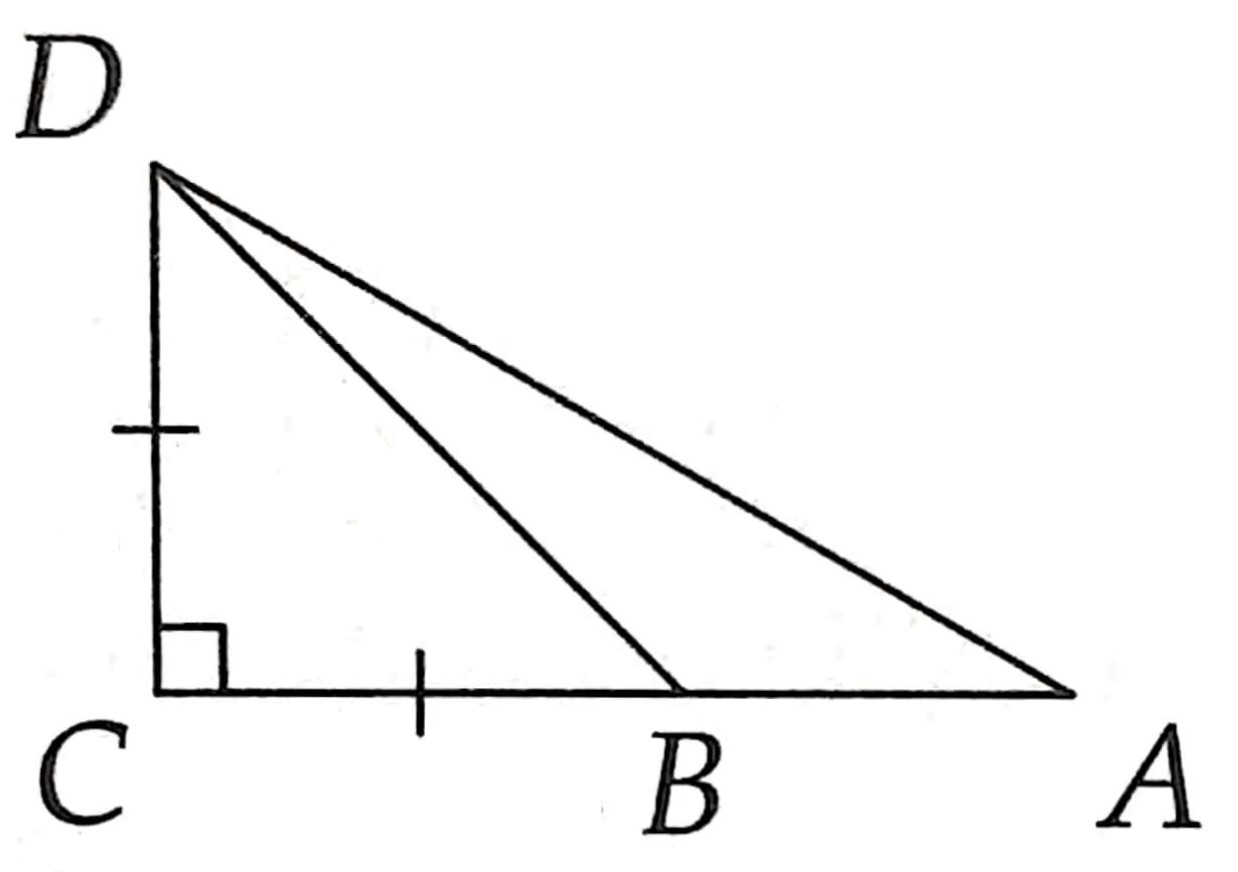
\includegraphics[width=4cm]{img1.jpg}
    \end{figure}
    
    %ans: c 3/2
    $\textbf{(A)}\ \frac{12-6\sqrt{3}}{\sqrt{3}-1} \qquad \textbf{(B)}\ \frac{9-3\sqrt{3}}{\sqrt{3}-1} \qquad \textbf{(C)}\ \frac{3}{2}\qquad \textbf{(D)}\ \frac{2}{3}\qquad \textbf{(E)}\ 3$
        
    % 10
     \item In an alternate universe, McDonalds sells Chicken McNuggets in packets of 3 and 5. Some wise person (Kevin) wonders what the largest number of Chicken McNuggets that one can't buy is. Help Kevin confuse the McDonalds staff.
    
    %Ans: D
    $\textbf{(A)}\ 14 \qquad \textbf{(B)}\ 11 \qquad \textbf{(C)}\ 4 \qquad \textbf{(D)}\ 7 \qquad \textbf{(E)}\ 2$
    \end{enumerate}


\par\noindent\rule[0.5]{\textwidth}{1pt}
\\\\\textbf{Part B: Each correct answer is worth 6.}
    \begin{enumerate}
        \setcounter{enumi}{10}
    % 11
    \item A pen and a pencil originally sold for $30$ dollars and $60$ dollars, respectively. During a sale Eric bought the $30$ dollar pen at a $20\%$ discount and the $60$ dollar pencil at a $35\%$ discount. The total amount saved was what percent of the total of the original prices?
    
    % ans: B: 30%
    $\textbf{(A)}\ 25\% \qquad \textbf{(B)}\ 30\% \qquad \textbf{(C)}\ 35\% \qquad \textbf{(D)}\ 40\% \qquad \textbf{(E)}\ 45\%$
    
    % 12
    \item A box of cards contains $5$ cards, numbered $1$, $2$, $3$, $4$, and $5$. Cards are then drawn randomly one at a time without replacement until the sum of the values drawn exceeds $4$. What is the probability that $3$ card draws are required?
    
    % ans: D: 1/5
     $\textbf{(A)}\ \frac{1}{15} \qquad \textbf{(B)}\ \frac{1}{10} \qquad \textbf{(C)}\ \frac{1}{6} \qquad \textbf{(D)}\ \frac{1}{5} \qquad \textbf{(E)}\ \frac{1}{4}$
    
    % 13
     \item Dr. Muzsi is famous for his Christmas parties. This year, 40 lucky guests were invited. There are 35 people who all know each other and 5 people who know no one (except Dr. Muzsi of course). People who know each other hug, and people who do not know each other shake hands. As the banquet's host, Dr. Muzsi knows everyone. How many handshakes occur?
     
    %ans: C: 185
    $\textbf{(A)}\ 175 \qquad \textbf{(B)}\ 195 \qquad \textbf{(C)}\ 185\qquad \textbf{(D)}\ 350\qquad \textbf{(E)}\ 360$
        
    % 14
     \item Let $f$ be a function with the following properties:
    \begin{enumerate}
        \item $f(1) = 1$, and
        \item $f(2n) = n\times f(n)$, for any positive integer $n$.
    \end{enumerate}
    What is the value of $f(2^{100})$?

    % ans: D
    $\textbf{(A)}\ 1 \qquad \textbf{(B)}\ 2^{99} \qquad \textbf{(C)}\ 2^{100} \qquad \textbf{(D)}\ 2^{4950} \qquad \textbf{(E)}\ 2^{9999}$
        
    % 15
     \item Points $B,O,M$ and $C$ lie on a line, in that order, with $BO = MC$ and $OM = 12$. Point $D$ is not on the line, and $OD = MD = 10$. The perimeter of $\triangle BDC$ is twice the perimeter of $\triangle ODM$. Find $BO$.

    $\textbf{(A)}\ \frac{15}{2} \qquad \textbf{(B)}\ 8 \qquad \textbf{(C)}\ \frac{17}{2}\qquad \textbf{(D)}\ 9\qquad \textbf{(E)}\ \frac{19}{2}$
        
    % 16 
     \item If $\sin(x) =3 \cos(x)$ then what is $\sin(x) \cdot \cos(x)$?

    % ans: E
    $\textbf{(A)}\ \frac{1}{6} \qquad \textbf{(B)}\ \frac{1}{5} \qquad \textbf{(C)}\ \frac{2}{9}\qquad \textbf{(D)}\ \frac{1}{4}\qquad \textbf{(E)}\ \frac{3}{10}$
        
    % 17
     \item For how many positive integer values of $n$ are $\frac{n}{3}$ and $3n$ both three-digit whole numbers?

    %ans: A: 12
    $\textbf{(A)}\ 12 \qquad \textbf{(B)}\ 21 \qquad \textbf{(C)}\ 27 \qquad \textbf{(D)}\ 33 \qquad \textbf{(E)}\ 34$
    
    % 18
    \item For nonzero constants c and d, the equation $4x^3 - 12x^2 + cx + d = 0$ has two real roots which add to give 0. Find $\frac{d}{c}$.
    
    %ans E -3
    $\textbf{(A)}\ -1 \qquad \textbf{(B)}\ -12 \qquad \textbf{(C)}\ 12\qquad \textbf{(D)}\ 3\qquad \textbf{(E)}\ -3$
        
    % 19
     \item Find $x^4 +\frac{1}{x^4}$ if $x-\frac{1}{x}=5.$

    %Ans: D 727
    $\textbf{(A)}\ 531 \qquad \textbf{(B)}\ 527 \qquad \textbf{(C)}\ 731\qquad \textbf{(D)}\ 727\qquad \textbf{(E)}\ 729$
        
    % 20
     \item What is the minimum value of $f(x,y) = x^2 - 4x + y^2 + 6y$ when x and y are subjected to the restrictions $0 \leq x \leq 1$ and $0 \leq y \leq 1$?

    % ans: E -3
     $\textbf{(A)}\ 0 \qquad \textbf{(B)}\ -1 \qquad \textbf{(C)}\ 1 \qquad \textbf{(D)}\ -2 \qquad \textbf{(E)}\ -3 $
    \end{enumerate}
    
\par\noindent\rule{\textwidth}{1pt}
\\\\\textbf{Part C: Each correct answer is worth 8.}
     \begin{enumerate}
        \setcounter{enumi}{20}
    % 21
    \item In $\triangle ABC, \angle C = 90\degree, AC = 12,$ and $AB = 13.$ Point $M$ lies on $AC$ and point $N$ lies on hypotenuse $AB$ such that $AM = MN = NB.$ Compute $AM.$
    
    % ans: A 169/37
     $\textbf{(A)}\ \frac{169}{37} \qquad \textbf{(B)}\ \frac{13}{37} \qquad \textbf{(C)}\ \frac{13}{1369}\qquad \textbf{(D)}\ 3 \qquad \textbf{(E)}\ \frac{169}{1369}$
     
    % 22
    \item Find the largest possible value of x, where x and y are positive integers, that satisfies the equation, $1! + 2! + 3! + ... + x! = y^2$.
    
    % ans: E 3
     $\textbf{(A)}\ 89350\qquad \textbf{(B)}\ 43854\qquad \textbf{(C)}\ 34433\qquad \textbf{(D)}\ 65392 \qquad \textbf{(E)}\ 3 $
     
    % 23
    \item The equations $x^3 + Ax + 10 = 0$ and $x^3 + Bx^2 + 50 = 0$ have two roots in common. Compute the product of these common roots.
    
    % ans: C
     $\textbf{(A)}\ 4\sqrt[3]{2} \qquad \textbf{(B)}\ \frac{5\sqrt[3]{4}}{4} \qquad \textbf{(C)}\ 5\sqrt[3]{4}\qquad \textbf{(D)}\ \frac{13}{4} \qquad \textbf{(E)}\ -10$
     
    % 24
    \item Find the sum of all positive integers $n$ such that when $1^3+2^3+3^3+\cdots +n^3$ is divided by $n+5$, the remainder is $17$.
    
    % ans: B 239
     $\textbf{(A)}\ 566\qquad \textbf{(B)}\ 239\qquad \textbf{(C)}\ 420\qquad \textbf{(D)} 643\  \qquad \textbf{(E)}\ 359$
     
    % 25
    \item There is a unique square $S$ such that each of the four points $B(0,12), O(10,9), M(8,0),$ and $C(-4,7).$ are on a different side of $S$. Let $K$ be the area of $S$. Find the remainder when $10K$ is divided by $1000$.
    
    % ans: D 936
     $\textbf{(A)}\ 972 \qquad \textbf{(B)}\ 967 \qquad \textbf{(C)}\ 420\qquad \textbf{(D)}\ 936 \qquad \textbf{(E)}\ 944 $

\end{enumerate}

%Message

\newpage

\begin{center}
       
\includegraphics[width=10cm]{Bur Oak Math Club Banner Bold.png}
\end{center}

\subsection*{To Participants:}
Thank you so much for writing the BOMC '20 December Contest! This is the first ever BOMC Math Contest ever! Every month, we, the BOMC team, intends to bring you yet another contest for you to compete in. We encourage you to participate each month to prepare yourself for contests like the AMC, COMC, and Waterloo contests.\bigskip

Visit our \href{https://discord.gg/QkdPFaNxgQ}{Discord Server} to...
\begin{itemize}
    \item Participate in future BOMC contests.
    \item Practice worksheets to help you learn more mathematics and prepare for future contests.
    \item Attend Zoom lessons on various Math Olympiad topics.
    \item Talk with other students interested in math.
    \item View your contest results.
\end{itemize}

\subsection*{Mini Survey:}
Tell us how the contest went! Send us an email at buroakmatholympiads@gmail.com. Your email can comment on some of these items or anything else you have to say:
\begin{itemize}
    \item The overall difficulty of the handout. (Were there problems that were too easy or hard for their point value?)
    \item Were there any lame, niche, or weird problems? 
    \item Was the wording easy to understand?
    \item What do you think about the format of the test? (point system, problems per section, etc.)
\end{itemize}

The more feedback we receive about the BOMC contest, the better. Your feedback will greatly help us improve future BOMC contests. And don't worry for being informal in your email - all feedback is appreciated!


\end{document}
